\documentclass{article}
\usepackage[utf8]{inputenc}
\usepackage{adjustbox}
\usepackage[utf8]{inputenc}
\usepackage[margin=1in]{geometry}
\usepackage{graphicx}

\title{Herramientas Computacionales: Trabajo Practico N°2}
\author{Mateo Freile & Juan Pablo Pedregal }
\date{07/04/2021}

\begin{document}

\maketitle

\section{Chicago}
Los siguientes 3 mapas  coropléticos muestran al estado de Chicago dividido por departamentos. En particular, el primer mapa los presenta pintados de un color más rojizo a los que tienen precios promedio de alquiler en Airbnb en dólares por persona en octubre de 2015 más altos que los pintados en tonos más claros.\\
El segundo mapa representa gráficamente cuanto es el ingreso promedio por persona en cada departamento. La elección de colores es análoga al primer gráfico, es decir, los colores se vuelven rojizos conforme aumenta el ingreso.\\
El tercer mapa muestra la cantidad de crímenes cada mil habitantes por departamento. Los crímenes son entendidos como: agresión, asalto, juegos de azar, homicidio, secuestro, robo, acecho y hurto, desde octubre de 2014 a septiembre de 2015.\\
Comparando los tres mapas parecería que la zona norte tiene los precios e ingresos más altos y menos crímenes que la zona sur, con excepción de algunos estados.\\
En el primer gráfico de puntos notamos una tenue correlación positiva entre los ingresos y los precios, mientras que la correlación entre crímenes y precios parece ser nula en el segundo gráfico.\\
El último gráfico es un box plot sobre los precios. Se puede apreciar el valor mínimo, mediano y máximo que toma dicha variable. También que el 50 \% de los datos se encuentran entre los 52,65 y 87,32 dólares.

%Primera Imagen
\begin{figure}[htbp]
\centerline{\includegraphics[scale=.4]{Precios por persona-2.png}}
\caption{}
\label{fig}
\end{figure}\\


%Segunda Imagen
\begin{figure}[htbp]
\centerline{\includegraphics[scale=.4]{Ingreso pér cápita.png}}
\caption{}
\label{fig}
\end{figure}

%Tercera Imagen
\begin{figure}[htbp]
\centerline{\includegraphics[scale=.4]{Cantidad de Crímenes cada 1000 habitantes.png}}
\caption{}
\label{fig}
\end{figure}

%Cuarta Imagen
\begin{figure}[htbp]
\centerline{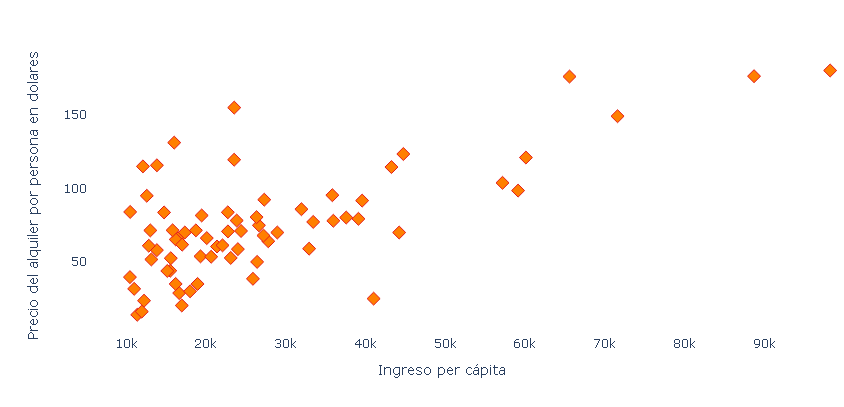
\includegraphics[scale=.75]{Precios contra Ingreso.png}}
\caption{}
\label{fig}
\end{figure}

%Quinta Imagen
\begin{figure}[htbp]
\centerline{\includegraphics[scale=1]{Precios contra Crímenes.png}}
\caption{}
\label{fig}
\end{figure}


%Sexta Imagen
\begin{figure}[htbp]
\centerline{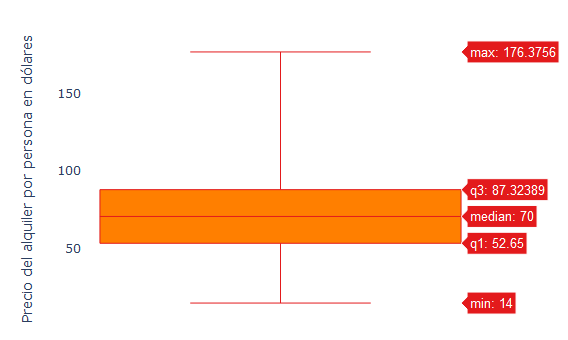
\includegraphics[scale=1]{Box Plot de precios.png}}
\caption{}
\label{fig}
\end{figure}

\section{Buenos Aires}
El primer mapa de la provincia de Buenos Aires junto con CABA muestra el porcentaje de hogares con necesidades básicas insatisfechas (NBI).Curiosamente, excepto casos excepcionales (Lobería, Necochea, San Cayetano, Tres Arroyos y Coronel Dorrego), se puede observar que aquellos municipios ubicados en la costa poseen mayor porcentaje de hogares con NBI con respecto a los ubicados en el centro de la provincia. Específicamente el área comprendida entre Cañuelas, Berisso, Pilar y San Fernando junto con Zarate, Villarino y Patagones poseen un porcentaje entre 9,12 y 18,36.\\

El segundo mapa muestra el porcentaje de desocupados, ambos medidos en el censo nacional de 2010.Exceptuando algunos casos (Coronel Pringles, Adolfo Alsina, Olavarría, Azul, Benito Juárez, Tandil y Balcarce) pareceria repetirse el mismo resultado del gráfico anterior, en donde aquellos municipios localizados cerca de la costa presentan los mayores porcentajes de desocupación.



%FIGURA 7
\begin{figure}[htbp]
\centerline{\includegraphics[scale=.3]{_ de Hogares con NBI.png}}
\caption{}
\label{fig}
\end{figure}

%FIGURA 8
\begin{figure}[htbp]
\centerline{\includegraphics[scale=.3]{DESOCUPADOS.png}}
\caption{}
\label{fig}
\end{figure}






\end{document}






